% This file was created by matplotlib v0.1.0.
% Copyright (c) 2010--2014, Nico Schlömer <nico.schloemer@gmail.com>
% All rights reserved.
%
% The lastest updates can be retrieved from
%
% https://github.com/nschloe/matplotlib2tikz
%
% where you can also submit bug reports and leavecomments.
%
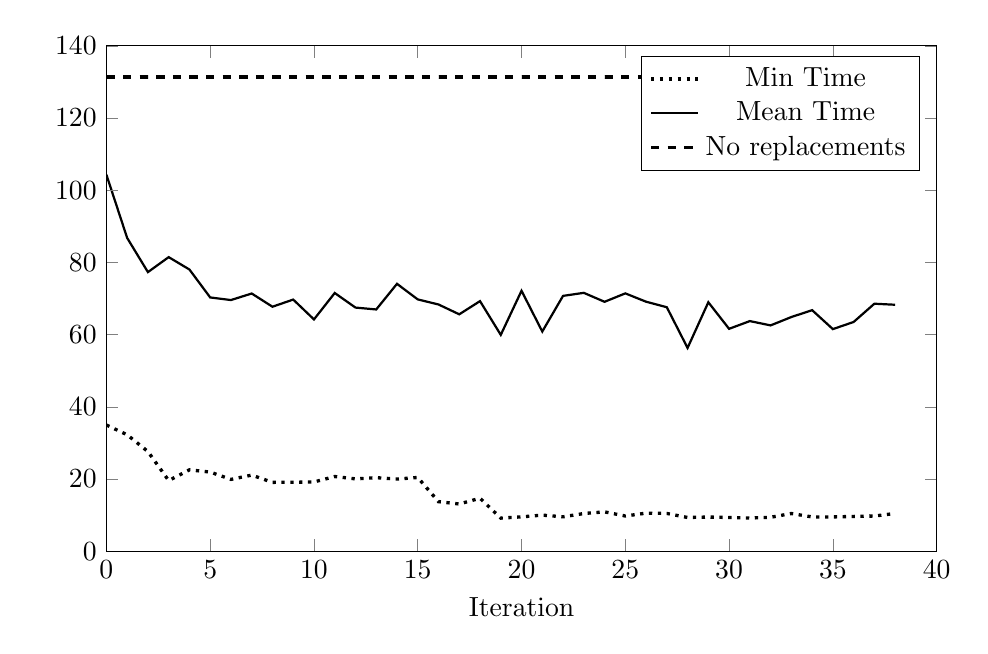
\begin{tikzpicture}[trim left=-1cm]

\begin{axis}[
width=\textwidth,
height=8cm,
xlabel={Iteration},
xmin=0, xmax=40,
ymin=0, ymax=140,
axis on top,
legend entries={{Min Time},{Mean Time},{No replacements}}
]
\addplot [dotted, very thick]
coordinates {
(0,34.9579)
(1,32.254)
(2,27.608)
(3,19.5639)
(4,22.5339)
(5,21.9218)
(6,19.8978)
(7,21.0829)
(8,19.074)
(9,19.0999)
(10,19.1823)
(11,20.69)
(12,20.0326)
(13,20.3687)
(14,19.9832)
(15,20.4251)
(16,13.7228)
(17,13.078)
(18,14.6786)
(19,9.16225)
(20,9.51277)
(21,9.99713)
(22,9.53025)
(23,10.4417)
(24,10.8963)
(25,9.75238)
(26,10.5461)
(27,10.4678)
(28,9.34168)
(29,9.46352)
(30,9.33624)
(31,9.18503)
(32,9.39811)
(33,10.4357)
(34,9.49689)
(35,9.497)
(36,9.63368)
(37,9.74072)
(38,10.4566)

};
\addplot [thick]
coordinates {
(0,104.295644)
(1,86.773332)
(2,77.310664)
(3,81.463924)
(4,78.032816)
(5,70.292842)
(6,69.572714)
(7,71.385022)
(8,67.725246)
(9,69.707306)
(10,64.206444)
(11,71.526236)
(12,67.486658)
(13,66.966018)
(14,74.072268)
(15,69.747516)
(16,68.344832)
(17,65.621184)
(18,69.279372)
(19,59.927595)
(20,72.1396894)
(21,60.8503046)
(22,70.727957)
(23,71.572178)
(24,69.088654)
(25,71.4234876)
(26,69.115268)
(27,67.582904)
(28,56.3051556)
(29,68.9650784)
(30,61.6033428)
(31,63.7455946)
(32,62.5515042)
(33,64.86731)
(34,66.7744258)
(35,61.524602)
(36,63.4963436)
(37,68.5563764)
(38,68.269344)

};
\addplot [dashed, very thick]
coordinates {
(0,131.376)
(1,131.376)
(2,131.376)
(3,131.376)
(4,131.376)
(5,131.376)
(6,131.376)
(7,131.376)
(8,131.376)
(9,131.376)
(10,131.376)
(11,131.376)
(12,131.376)
(13,131.376)
(14,131.376)
(15,131.376)
(16,131.376)
(17,131.376)
(18,131.376)
(19,131.376)
(20,131.376)
(21,131.376)
(22,131.376)
(23,131.376)
(24,131.376)
(25,131.376)
(26,131.376)
(27,131.376)
(28,131.376)
(29,131.376)
(30,131.376)
(31,131.376)
(32,131.376)
(33,131.376)
(34,131.376)
(35,131.376)
(36,131.376)
(37,131.376)
(38,131.376)

};
\path [draw=black, fill opacity=0] (axis cs:13,140)--(axis cs:13,140);

\path [draw=black, fill opacity=0] (axis cs:40,13)--(axis cs:40,13);

\path [draw=black, fill opacity=0] (axis cs:13,0)--(axis cs:13,0);

\path [draw=black, fill opacity=0] (axis cs:0,13)--(axis cs:0,13);

\end{axis}

\end{tikzpicture}
